%% Relatório final — formato ACM sigconf (limite: 2 páginas, sem contar referências,
%% declaração de uso de IA e declaração de contribuição).
%% Compilar com o acmart.cls de ACM_Conference_Proceedings_Primary_Article_Template/
%% (ou no Overleaf): pdflatex main && bibtex main && pdflatex main && pdflatex main
\documentclass[sigconf,nonacm]{acmart}
\usepackage[brazilian]{babel}
\usepackage{booktabs}
\settopmatter{printacmref=false,printfolios=false}
\setcopyright{none}
\renewcommand\footnotetextcopyrightpermission[1]{}
\AtBeginDocument{\providecommand\BibTeX{{Bib\TeX}}}

\newcommand{\ci}[2]{\,[#1;\,#2]}

\begin{document}

\title{LLMs de uso geral ou um classificador calibrado? A confiança do Jev em português em três tarefas de classificação}

%% Autores num único bloco com afiliação compartilhada (economiza espaço no topo).
\author{Bernardo Machado, Guilherme Ferreira, Luísa Porfírio, Marco Túlio Marcelino e Túlio de Sousa}
\affiliation{\institution{Universidade Federal de Minas Gerais}\city{Belo Horizonte}\country{Brasil}}
\renewcommand{\shortauthors}{Machado et al.}

\begin{abstract}
LLMs de uso geral classificam mensagens, mas sua confiança, pedida por escrito, tende a ser exagerada, o que limita quanto se pode automatizar. O Jev (TypeSafe AI) apenas escolhe entre opções fixas e devolve probabilidades descritas como calibradas. Comparamos o Jev com dois LLMs abertos locais (Ministral-3 14B e Gemma-4-E4B) e três via API (DeepSeek-V4.1-Flash, DeepSeek-V4-Pro e Gemini 3.1 Flash-Lite) em três bases (intenções bancárias, pedidos a assistentes virtuais e tópicos de frases), em inglês e em português. Em português, o Jev é mais bem calibrado que o Ministral nas três bases e que os LLMs via API na base bancária, a de classes mais próximas; nas outras duas, eles o igualam. Em todas, a confiança do Jev é a que melhor separa acertos de erros, o que permite automatizar mais mensagens com a mesma exigência de acerto. Não detectamos efeito consistente da troca de idioma na calibração (ICs com meia-largura de cerca de 0,03 de ECE).
\end{abstract}

\maketitle

\section{Problema e motivação}
Em atendimento automatizado, cada mensagem que precisa passar por um humano tem um \emph{custo por toque}. Um classificador reduz esse custo quando sua confiança indica quais respostas podem ser aceitas sem revisão, o que exige \emph{calibração}: entre as respostas dadas com 90\% de confiança, cerca de 90\% devem estar certas~\cite{guo2017calibration}. Medimos o desvio com o erro de calibração esperado (ECE), a diferença média entre confiança e acurácia em faixas de confiança (0 é calibração perfeita)~\cite{naeini2015ece}.

A solução mais comum hoje é um LLM generativo: o prompt lista as opções e pede-se que o modelo escreva também um número entre 0 e 1 (confiança \emph{verbalizada}), de calibração variável~\cite{tian2023justask,xiong2024uncertainty}. O Jev segue outro desenho: não gera texto, só escolhe entre opções fixas e devolve uma probabilidade para cada uma, a US\$\,0,042 por milhão de tokens de entrada; seu benchmark cobre 37 bases~\cite{deusser2026jev}, nenhuma com entradas em português. Perguntamos: \textbf{Q1} (hipótese H1, definida antes dos experimentos): em português, o ECE do Jev é menor que o do Ministral-3 14B com confiança verbalizada? \textbf{Q2}: a calibração muda do inglês para o português? \textbf{Q3}: em português, quantas mensagens cada sistema permite automatizar sem perder acurácia, e a que custo?

\begin{figure}[t]
  \centering
  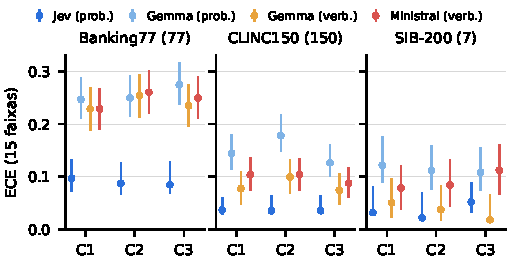
\includegraphics[width=\linewidth]{figs/ece_datasets.pdf}
  \caption{ECE (15 faixas) e IC 95\% por base (nº de opções), sistema e condição.}
  \label{fig:ece}
\end{figure}

\begin{table*}[t]
  \caption{ECE em C3 e $\Delta$ECE pareado [IC 95\%] nos itens válidos em ambos; negativo favorece o primeiro.}
  \label{tab:h1}
  \footnotesize
  \begin{tabular}{lcccc}
    \toprule
     & Banking77 & CLINC150 & SIB-200 & Média \\
    \midrule
    ECE Jev / Ministral / Gemma verb. / prob. & 0,085 / 0,250 / 0,235 / 0,275 & 0,036 / 0,088 / 0,074 / 0,127 & 0,052 / 0,112 / 0,018 / 0,109 & 0,058 / 0,150 / 0,109 / 0,170 \\
    ECE DeepSeek Flash / Pro / Gemini & 0,114 / 0,185 / 0,184 & 0,018 / 0,041 / 0,057 & 0,042 / 0,028 / 0,061 & 0,058 / 0,084 / 0,101 \\
    \midrule
    $\Delta$ Jev $-$ Ministral (H1) & $-$0,165\ci{$-$0,189}{$-$0,120} & $-$0,053\ci{$-$0,070}{$-$0,014} & $-$0,063\ci{$-$0,101}{$-$0,011} & $-$0,093\ci{$-$0,105}{$-$0,062} \\
    $\Delta$ Jev $-$ Gemma verb. & $-$0,148\ci{$-$0,173}{$-$0,101} & $-$0,039\ci{$-$0,058}{0,000} & $+$0,034\ci{$-$0,012}{0,054} & $-$0,051\ci{$-$0,067}{$-$0,029} \\
    $\Delta$ Jev $-$ Gemma prob. & $-$0,190\ci{$-$0,218}{$-$0,143} & $-$0,091\ci{$-$0,114}{$-$0,054} & $-$0,057\ci{$-$0,095}{$-$0,015} & $-$0,112\ci{$-$0,127}{$-$0,085} \\
    $\Delta$ Jev $-$ DeepSeek Flash & $-$0,029\ci{$-$0,048}{0,011} & $+$0,018\ci{$-$0,001}{0,043} & $+$0,010\ci{$-$0,035}{0,037} & $-$0,000\ci{$-$0,016}{0,019} \\
    $\Delta$ Jev $-$ DeepSeek Pro & $-$0,100\ci{$-$0,120}{$-$0,057} & $-$0,005\ci{$-$0,021}{0,027} & $+$0,024\ci{$-$0,022}{0,052} & $-$0,027\ci{$-$0,041}{$-$0,005} \\
    $\Delta$ Jev $-$ Gemini & $-$0,099\ci{$-$0,118}{$-$0,058} & $-$0,022\ci{$-$0,034}{0,012} & $-$0,009\ci{$-$0,040}{0,022} & $-$0,043\ci{$-$0,052}{$-$0,020} \\
    $\Delta$ Gemma verb. $-$ prob. & $-$0,042\ci{$-$0,077}{$-$0,010} & $-$0,052\ci{$-$0,079}{$-$0,031} & $-$0,090\ci{$-$0,113}{$-$0,035} & --- \\
    \bottomrule
  \end{tabular}
\end{table*}

\section{Abordagem}
\textbf{Sistemas.} (i) \emph{Jev} (1.14.0, via API): a confiança é a probabilidade da opção escolhida. (ii) \emph{Ministral-3 14B}, LLM aberto local (Ollama, 4 bits, temperatura 0), que responde em JSON a intenção e a confiança. (iii) \emph{Gemma-4-E4B}, em bf16 como no benchmark, lido de duas formas, o que separa modelo e forma de leitura: \emph{prob.}, em que cada opção recebe um código de um único token e a confiança é a probabilidade do próximo token, renormalizada sobre os códigos (método do benchmark~\cite{deusser2026jev}); e \emph{verb.}, com o prompt do Ministral. O Ministral representa o uso prático, quantizado. O Qwen3.8-27B previsto não foi executado: em bf16 não cabe nos 48\,GB da GPU. (iv) Acrescentados após a execução principal (exploratório, fora de H1), com o prompt do Ministral: \emph{DeepSeek-V4.1-Flash} e \emph{V4-Pro} (API, 17/11/2026, sem raciocínio, temperatura 0) e \emph{Gemini 3.1 Flash-Lite} (API, raciocínio baixo).

\textbf{Condições.} C1: tudo em inglês. C2: só a mensagem em português, isolando o idioma do conteúdo (contraste principal de Q2). C3: tudo em português, o uso real e a condição de H1.

\textbf{Bases.} \emph{Banking77}~\cite{casanueva2020banking77}: mensagens de clientes de banco em 77 intenções muito próximas; 6 por intenção, com tradução revisada por humanos~\cite{dimant2025banking77pt}. \emph{CLINC150}~\cite{larson2019clinc}: pedidos a assistentes virtuais em 150 intenções de 10 domínios, sem a classe fora de escopo; 3 por intenção, com tradução automática não revisada~\cite{tech4humans_clinc_pt}. \emph{SIB-200}~\cite{adelani2024sib}: frases em 7 tópicos; o teste inteiro (204), com a tradução profissional do FLORES-200~\cite{nllb2022}. As amostras foram estratificadas por classe (semente 42), por limite de tempo de GPU.

\textbf{Métricas.} Primária: ECE com 15 faixas, fixadas antes da execução (10, 20 e 30 como verificação). Secundárias: acurácia, AURC (área sob a curva do erro em função da fração de respostas aceitas; menor é melhor)~\cite{geifman2017selective} e fração de mensagens automatizável mantendo 90\% ou 95\% de acerto. ICs de 95\% vêm de \emph{bootstrap} pareado (5.000 reamostragens dos mesmos itens para os dois sistemas). H1 é apoiada se todo o IC de ECE$_{\text{Jev}}-$ECE$_{\text{Ministral}}$ ficar abaixo de zero; médias entre bases dão peso igual a cada uma.

\textbf{Execução.} Cada sistema classificou 1.116 itens nas três condições: os LLMs abertos numa GPU NVIDIA L40S, os demais pelas APIs. Respostas fora da lista de opções (menos de 1\%) foram descartadas, e cada comparação pareada usa os itens válidos nos dois sistemas. \textbf{Validação:} em inglês, no Banking77, obtivemos para o Jev acurácia 0,784 \ci{0{,}745}{0{,}823} e ECE 0,097 \ci{0{,}073}{0{,}132}, contra 0,797 e 0,087 publicados~\cite{deusser2026jev}; para o Gemma \emph{prob.}, 0,673 e 0,247, contra 0,670 e 0,267. Código, prompts e respostas brutas: \url{https://github.com/guiinow/Jev-LLM-callibration}.

\begin{table}[t]
  \caption{Acurácia em inglês e $\Delta$ECE ao passar ao português (* IC 95\% exclui zero; ICs no repositório).}
  \label{tab:q2}
  \setlength{\tabcolsep}{4pt}
  \resizebox{\linewidth}{!}{%
  \begin{tabular}{l ccc ccc ccc}
    \toprule
    & \multicolumn{3}{c}{Banking77} & \multicolumn{3}{c}{CLINC150} & \multicolumn{3}{c}{SIB-200} \\
    \cmidrule(lr){2-4}\cmidrule(lr){5-7}\cmidrule(lr){8-10}
    Sistema & Ac.\,C1 & C2$-$C1 & C3$-$C1 & Ac.\,C1 & C2$-$C1 & C3$-$C1 & Ac.\,C1 & C2$-$C1 & C3$-$C1 \\
    \midrule
    Jev        & 0,784 & $-$0,010 & $-$0,012 & 0,936 & $-$0,001 & $-$0,001 & 0,907 & $-$0,010 & $+$0,020 \\
    Ministral  & 0,740 & $+$0,030* & $+$0,022 & 0,863 & $-$0,004 & $-$0,020 & 0,882 & $+$0,006 & $+$0,034 \\
    Gemma prob.& 0,673 & $+$0,003 & $+$0,028 & 0,807 & $+$0,034* & $-$0,018 & 0,843 & $-$0,010 & $-$0,013 \\
    Gemma verb.& 0,697 & $+$0,027* & $+$0,006 & 0,860 & $+$0,022 & $-$0,003 & 0,873 & $-$0,013 & $-$0,032 \\
    DS Flash   & 0,788 & $+$0,004 & $-$0,005 & 0,922 & $+$0,029* & $+$0,001 & 0,887 & $+$0,012 & $+$0,008 \\
    DS Pro     & 0,779 & $+$0,011 & $+$0,028* & 0,918 & $+$0,007 & $+$0,003 & 0,882 & $-$0,019 & $-$0,006 \\
    Gemini     & 0,779 & $+$0,013 & $+$0,006 & 0,927 & $-$0,001 & $+$0,004 & 0,892 & $-$0,012 & $+$0,004 \\
    \bottomrule
  \end{tabular}}
\end{table}

\section{Resultados}
\textbf{Q1 (H1).} Em português, o Jev é mais bem calibrado que o Ministral nas três bases, com ICs inteiramente abaixo de zero (Fig.~\ref{fig:ece}, Tab.~\ref{tab:h1}): H1 é apoiada, também com 10 a 30 faixas (exceto SIB-200 com 30) e em C1 e C2 (exceto SIB-200 em C1, inconclusivo). O Ministral é superconfiante: declara 95\% a 97\% de confiança em média para 71\% a 88\% de acerto; no Banking77 em português, 118 dos seus 127 erros têm confiança $\ge$90\%, contra 27 dos 94 do Jev.

\textbf{LLMs via API (exploratório).} São bem mais calibrados que o Ministral. O Flash iguala o Jev (diferenças inconclusivas nas três bases), e o Pro, maior, não é mais bem calibrado que ele; o Jev supera o Pro e o Gemini só no Banking77 e na média (Tab.~\ref{tab:h1}). No Banking77, 49 (Flash), 90 (Pro) e 78 (Gemini) dos seus 103 a 109 erros têm confiança $\ge$90\%.

\textbf{Modelo ou forma de leitura?} No Gemma, a confiança verbalizada é mais bem calibrada que a extraída das probabilidades nas três bases (Tab.~\ref{tab:h1}), e o Jev supera o Gemma \emph{verb.} claramente só no Banking77: sua vantagem não vem só da forma de leitura.

\textbf{Q2 (troca de idioma).} Das 42 variações (7 sistemas $\times$ 3 bases $\times$ 2 condições; Tab.~\ref{tab:q2}), só 5 têm IC que exclui zero, todas pequenas (até 0,034) e fora do Jev, compatíveis com o acaso sem correção para comparações múltiplas. Isso não prova equivalência: com ICs de meia-largura típica de 0,03 (0,02 no Jev), variações dessa ordem não seriam detectadas. A tradução afeta mais as respostas: o Jev muda a classe prevista em 2\% a 7\% dos itens, os LLMs via API em 2\% a 11\%, o Ministral em 8\% a 13\% e o Gemma em até 23\%.

\textbf{Q3 (seleção e custo por toque).} Em português, a AURC do Jev, que não depende de limiar, é a menor entre todos os sistemas nas três bases (Banking77: 0,078, contra 0,093 a 0,192). Exigindo 90\% de acerto, o Jev automatiza 70\% das mensagens do Banking77 e o Ministral, a 37\%; exigindo 95\%, o Jev automatiza 46\% do Banking77, 95\% do CLINC150 e 91\% do SIB-200, e o Ministral, 0\%, 62\% e 38\%. O 0\% vem de o Ministral usar quase só 0,95, 0,98 e 1,0, sem corte que isole 95\% de acerto. Com 95\%, os LLMs via API automatizam 0\% a 18\% do Banking77, 75\% a 86\% do CLINC150 e 18\% a 50\% do SIB-200. Os limiares foram escolhidos nos dados de teste, o que favorece todos. Mil classificações custam US\$\,0,04 a 0,07 no Jev (prompts de 1 a 1,7 mil tokens); custaram US\$\,0,04 (Flash) e US\$\,0,10 (Pro) na DeepSeek, com cache do prompt; o Ministral, em sequência numa L40S a US\$\,1,57/h (mediana de aluguel~\cite{getdeploying_l40s}; 0,56\,s por chamada), custaria US\$\,0,24, menos com lotes. O que pesa no custo por toque é a fração de mensagens que dispensa o humano.

% [SUPOSIÇÃO DE RASCUNHO: números da pré-anotação por LLM, tratada como já revisada pelo grupo; atualizar após a revisão]
\textbf{Análise de erros (Banking77, C3).} Os 221 erros do Jev (94) e do Ministral (127) receberam categorias sugeridas por um LLM e revisadas pelos autores, sem medida de concordância. Mais da metade dos erros do Jev (55\%) e 40\% dos do Ministral são de \emph{rótulo ambíguo}: a mensagem cabe em mais de uma intenção ou o rótulo é discutível; 29\% e 42\% confundem \emph{intenções próximas}, como transferência pendente e falha. A tradução quase nunca é a causa: 191 erros já ocorrem em inglês e, dos 28 que só aparecem em português, 3 se devem à tradução (p.ex.\ ``visa card'' virou ``cartão de crédito''). Com confiança $\ge$90\%, o Jev erra quase só em rótulos ambíguos (21 de 27); o Ministral, também em intenções próximas (50 de 118).

\section{Limitações e conclusões}
\textbf{Limitações.} Os LLMs abertos são pequenos, um quantizado em 4 bits; os via API entraram após a execução principal, com raciocínio desligado ou baixo, e as versões servidas podem mudar. Não avaliamos classificadores ajustados nem recalibração (p.ex.\ \emph{temperature scaling}), que reduziria o ECE dos LLMs; a AURC, porém, não muda sob recalibrações monotônicas. Com 204 a 462 itens o ECE é enviesado para cima, e várias faixas do Ministral ficam quase vazias. No CLINC150, idioma e qualidade da tradução (automática) se confundem; no Gemma, as duas leituras usam prompts diferentes.

\textbf{Conclusões.} Em português, o Jev foi mais bem calibrado que o Ministral nas três bases e que os demais LLMs no Banking77; nas outras bases, LLMs recentes via API o igualam. Em todas, sua confiança separou melhor acertos de erros e permitiu automatizar mais mensagens, a custo baixo e sem GPU própria. Não detectamos efeito consistente da troca de idioma na calibração.\label{fimcorpo}

\section*{Contribuições individuais}
% [A PREENCHER PELO GRUPO — não inferido pelo assistente]
Bernardo Machado: desenvolvimento dos experimentos. Guilherme Ferreira: definição da arquitetura do projeto, implementação dos métodos necessários para a experimentação inicial e disponibilização do repositório para trabalho distribuído. Luísa Porfírio: definição do escopo e da proposta do trabalho e desenvolvimento dos experimentos. Marco Túlio Marcelino: desenvolvimento e execução dos experimentos e escrita do relatório. Túlio de Sousa: desenvolvimento dos experimentos.

\section*{Declaração de uso de IA}
Ferramentas de IA generativa foram usadas como apoio na geração do código dos experimentos, na tradução para o português dos nomes das intenções do CLINC150, usados como opções em C3 (as mensagens das três bases vêm das traduções publicadas citadas na Seção~2), e na redação deste relatório. Todo o material produzido com esse apoio foi revisado pelo grupo, que é responsável pelo desenho experimental, pela validação dos resultados e pelas conclusões.

\bibliographystyle{ACM-Reference-Format}
\bibliography{references}

\end{document}
